\documentclass[a4paper, amsfonts, amssymb, amsmath, reprint, showkeys, nofootinbib, twoside]{revtex4-1}
\usepackage[english]{babel}
\usepackage[utf8]{inputenc}
\usepackage[colorinlistoftodos, color=green!40, prependcaption]{todonotes}
\usepackage[pdftex, pdftitle={Article}, pdfauthor={Author}]{hyperref}
\usepackage{amsthm}
\usepackage{mathtools}
\usepackage{physics}
\usepackage{xcolor}
\usepackage{caption}
\usepackage{hyperref}
%\hypersetup{colorlinks=true, linkcolor=blue, urlcolor = blue}
\usepackage{amsmath}
\usepackage{amssymb}
\usepackage{graphicx}
\graphicspath{Images}
\usepackage[left=23mm,right=13mm,top=35mm,columnsep=15pt]{geometry} 
\usepackage{adjustbox}
\usepackage{placeins}
\usepackage[T1]{fontenc}
\usepackage{float}
%\usepackage{longtable}
\usepackage{csquotes}
\usepackage{refstyle}
\usepackage{lipsum}

\begin{document}

\title{Study of Electronic Spin Resonance}
\author{Swaroop Ramakant Avarsekar}
\email{swaroop.avarsekar@niser.ac.in}
\affiliation{School of Physical Sciences, National Institute of Science Education and Research, HBNI, Jatni -752050, India}

	
\begin{abstract}
Electron Spin Resonance has been applied to the free radical 2,2 Diphenyl-1- picrylhydrazyl (DDPH) to determine the Lande's factor g. When the frequency of oscillation equal to the Larmor’s frequency of the sample, at resonance, the oscillator amplitude registers a dip due to the absorption of power by the sample, occurring four times in each complete cycle of Helmholtz coils supply voltage. From the two peaks obtained after changing the phase, distance between the peaks ($Q$) are calculated. With the different frequencies, $Q$ versus 1/$I$ is plotted to get the g factor to be 1.300 ± 0.068. 
\end{abstract}
	
\keywords{Resonance, Larmor's precession, Lande's factor}
	
\maketitle

\section{Introduction and Theory}
Electron Spin Resonance (ESR), also known as Electron Paramagnetic Resonance was  observed by Zavoisky in paramagnetic salts in 1945. ESR have been used as a tool for the study of radicals in solids. If a particle has magnetic moment $\mu$ placed in uniform magnetic field intensity $H_o$, then $\mu$ will precess around $H_o$ with an angular Larmor frequency $\omega_o$, given by the equation (\ref{e1}):

\begin{equation}\label{e1}
\omega_o=g\left(\frac{e}{2mc}\right)H_o
\end{equation}

where g is the Lande's factor. g=1 for the pure orbital momentum and g=2 for a free electron spin. For the case of anion in a crystal, the behaviour is modified by the environment and the $g$-factor may differ from the Lande's $g$-factor. This effective g- factor is known as the spectroscopic splitting factor. 

A weak magnetic field is introduced oriented in the X-Y plane and rotating about the z axis in the same direction as the Larmor precession with an angular
frequency $\omega_1$. If the frequency $\omega_1$ is different from $\omega_o$ the angle between the field $\vec{H_1}$ and the
magnetic moment $\mu$ will continuously change so that their interaction will average out to zero. If, however, $\omega_1$=$\omega_o$, the angle between $\vec{\mu}$ and $\vec{H_1}$ is maintained and net interaction is effective. If we look at the system in a reference frame that is rotating about the z axis with the
angular velocity $\vec{H_1}$ then the spin will appear to make an angle $90^{\circ}-\theta$ with $\vec{H_1}$, and according to the previous argument will start to precess (in the rotating frame) about $\vec{H_1}$. This corresponds to a nutation and a consequent change of the angle which implies a change in the potential energy of the particle in the magnetic field. The change in $\theta$ is the classical analogy to a transition between sub-levels with different m. We see that such transitions may take place only if the rotating field has an angular frequency $\omega_1$=$\omega_o$. 

In the quantum picture of elementary magnetic resonance, the intrinsic angular momentum of electron $\vec{s}$ couples with angular momentum $\vec{l}$ to give net as $\vec{j}$. \\$j$+1 magnetic sub-levels labelled by magnetic field $\vec{H_o}$ by equal energy difference :
\begin{equation}\label{e2}
\Delta E=g.\mu_o H_o
\end{equation}
This difference between adjacent sub-levels, whose correct quantum mechanical value is :
\begin{equation}
g=1+\frac{j(j+1)+s(s+1)-l(l+1)}{2j(j+1)}
\end{equation}

\begin{figure}[htbp] %  figure placement: here, top, bottom, or page
   \centering
   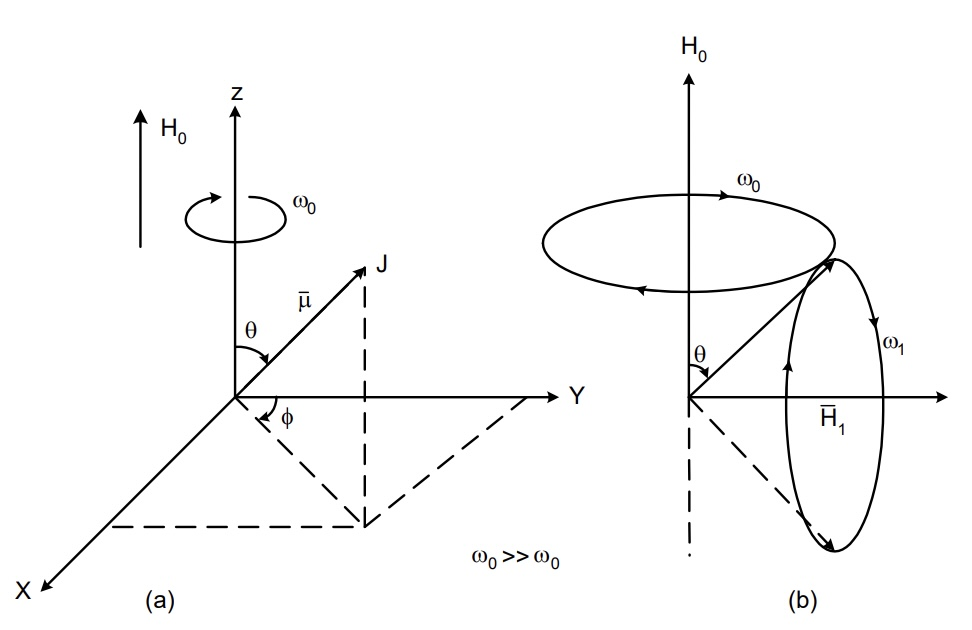
\includegraphics[width=8cm]{7} 
   \caption{(a) The spin precesses with angular frequency $\omega_o$, $\theta$ is constant throughout the motion. \newline (b) Weak magnetic field $\vec{H_1}$ is applied. $\vec{H_1}$ is rotating about z axis with angular frequency $\omega_o$, there $\mu$ precesses about $\vec{H_1}$ with angular frequency $\omega_1$ is not conserved.}
   \label{lp}
\end{figure}

If the particle is subjected to a perturbation by an alternating magnetic field with frequency $\nu_1$ with the direction perpendicular to the static magnetic field, then 
there will be induced transitions between neighbouring sub-levels
according to the selection rules $\Delta m=\pm1$ for magnetic dipolar radiation. 

Therefore at resonance, with $\nu_1$ is the resonance frequency.
\begin{equation}\label{69}
\Delta E=g.\mu_o H_o=h\nu_o=h\nu_1
\end{equation}

In atomic spectroscopy, transitions between sub-levels with different m. Instead the splitting of a level is observed through small change in frequency of the radiation emitted in the transition between widely distant levels. If the frequency corresponding to a transition between the sub-levels of the same state is measured, we get more precise value of energy splitting.

\section{Experiment}

\subsection{Apparatus}
\begin{figure}[htbp] %  figure placement: here, top, bottom, or page
   \centering
   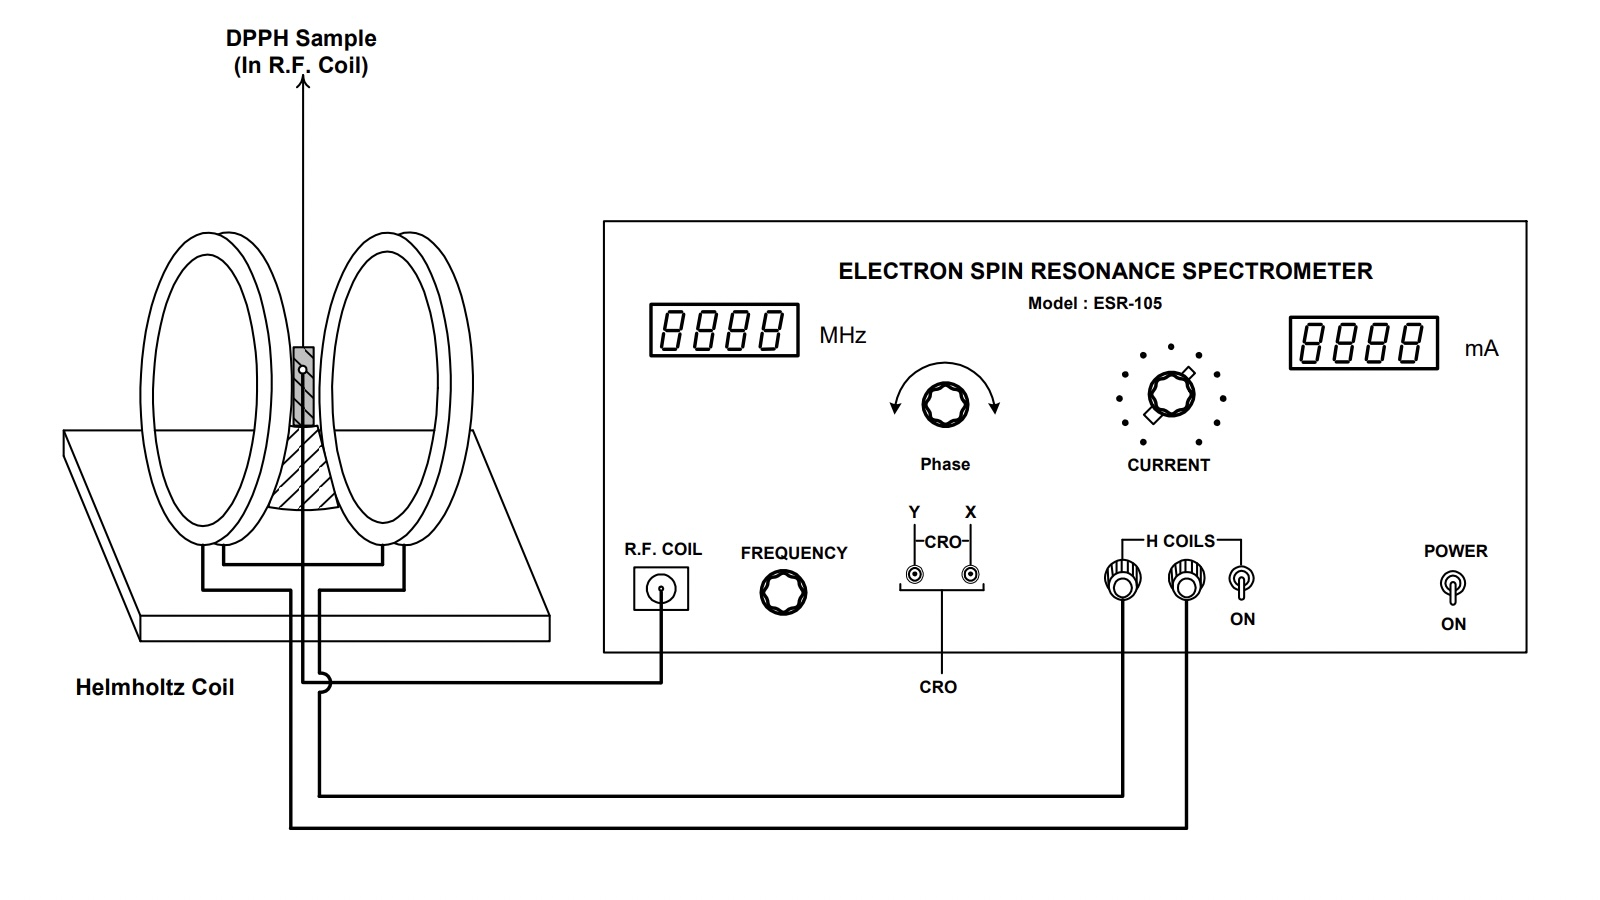
\includegraphics[width=8cm]{1} 
   \caption{Panel diagram of ESR spectrometer}
   \label{panel}
\end{figure}

\begin{figure}[htbp] %  figure placement: here, top, bottom, or page
   \centering
   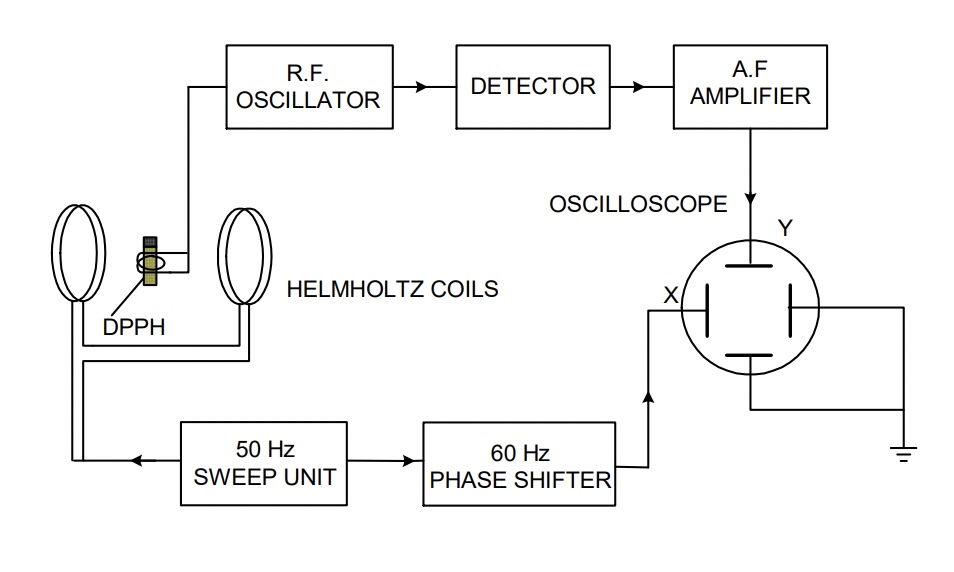
\includegraphics[width=8cm]{2} 
   \caption{Block diagram of ESR setup}
   \label{blok}
\end{figure}

The panel and block diagram of ESR spectrometer is given in Figure (\ref{panel}) and (\ref{blok}). The basic circuit consists of critically adjusted radio frequency oscillator with range 12-16 MHz. It is required so that slightest increase in the load decreases amplitude of oscillation to some extent. The sample used here is 2,2-Diphenyl-1-picrylhydrazyl (DDPH) in a plastic tube, which itself is in the induction coils, is kept in the 50 Hz magnetic field from Helmholtz coils. DDPH is a free radical ,as shown in Figure (\ref{dd}) and is widely used as standard ESR measurements. When the frequency of oscillation equal to the Larmor's frequency of the sample, at resonance, the oscillator amplitude registers a dip due to the absorption of power by the sample, occurring four times in each complete cycle of Helmholtz coils supply voltage. A phase shifter is used where the peaks could be seen in displaying type oscilloscope. For modulation with a low frequency magnetic field, a 50 Hz current flows through the Helmholtz coils. As the resonance in this frequency range occurs at low magnetic fields, no static D.C. magnetic field is required. ESR circuit requires highly stabilised voltage which can be obtained using integrated circuit regulator. 

\begin{figure}[htbp] %  figure placement: here, top, bottom, or page
   \centering
   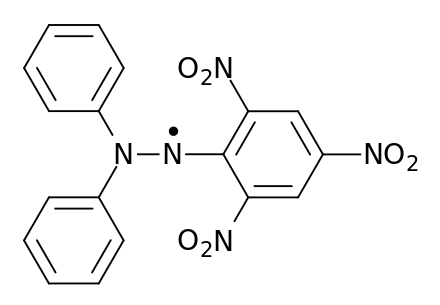
\includegraphics[width=5cm]{4} 
   \caption{2,2-Diphenyl-1-picrylhydrazyl (DDPH)}
   \label{dd}
\end{figure}

\subsection{Procedure}
To calibrate X plate of oscilloscope in terms of magnetic field, adjust the X amplifier of oscilloscope to obtain maximum, say $P$ divisions. From the current flowing in Helmholtz coils, calculate the magnetic field by:
\begin{equation}\label{q1}
H=\frac{32.\pi.n.I}{10.a\sqrt{125}}
\end{equation}
where $n$ is the no. of turns in each coil, $a$ is radius of the coils. 
H gives the rms field and peak to peak field will be $2\sqrt{2}H$, represent 'P' division of X plate. Zero field is at the middle point. Measure position of two peaks such that they are at equal distance $Q$. The magnetic field at the resonance is
\begin{equation}\label{q2}
H_o=\frac{2\sqrt{2}.H.Q}{P}
\end{equation}

Turn ON the Helmholtz coil and ESR spectrometer and adjust the current to about 150 mA and adjust the knob of frequency and phase towards the centre. Four peaks of signal could be seen in the oscilloscope; adjust the frequency and sensitivity of oscilloscope to get the sharp peaks and good signal to noise ratio. Adjust the phase such that the four peaks coincide to form two peaks. 

Raise the horizontal sensitivity of oscilloscope to maximum within the the linear range. Keeping the current say 150 mA initially, vary the current flowing through the coil with the frequency constant. Measure the distance between two peaks ($2Q$). Take five to six observations. Repeat the same procedure for different frequencies. Plot $\frac{1}{I}$ versus $Q$ and calculate the g factor using the $Q.I$ value from the graph. The experimental setup is as shown in Figure (\ref{setup})

\begin{figure}[htbp] %  figure placement: here, top, bottom, or page
   \centering
   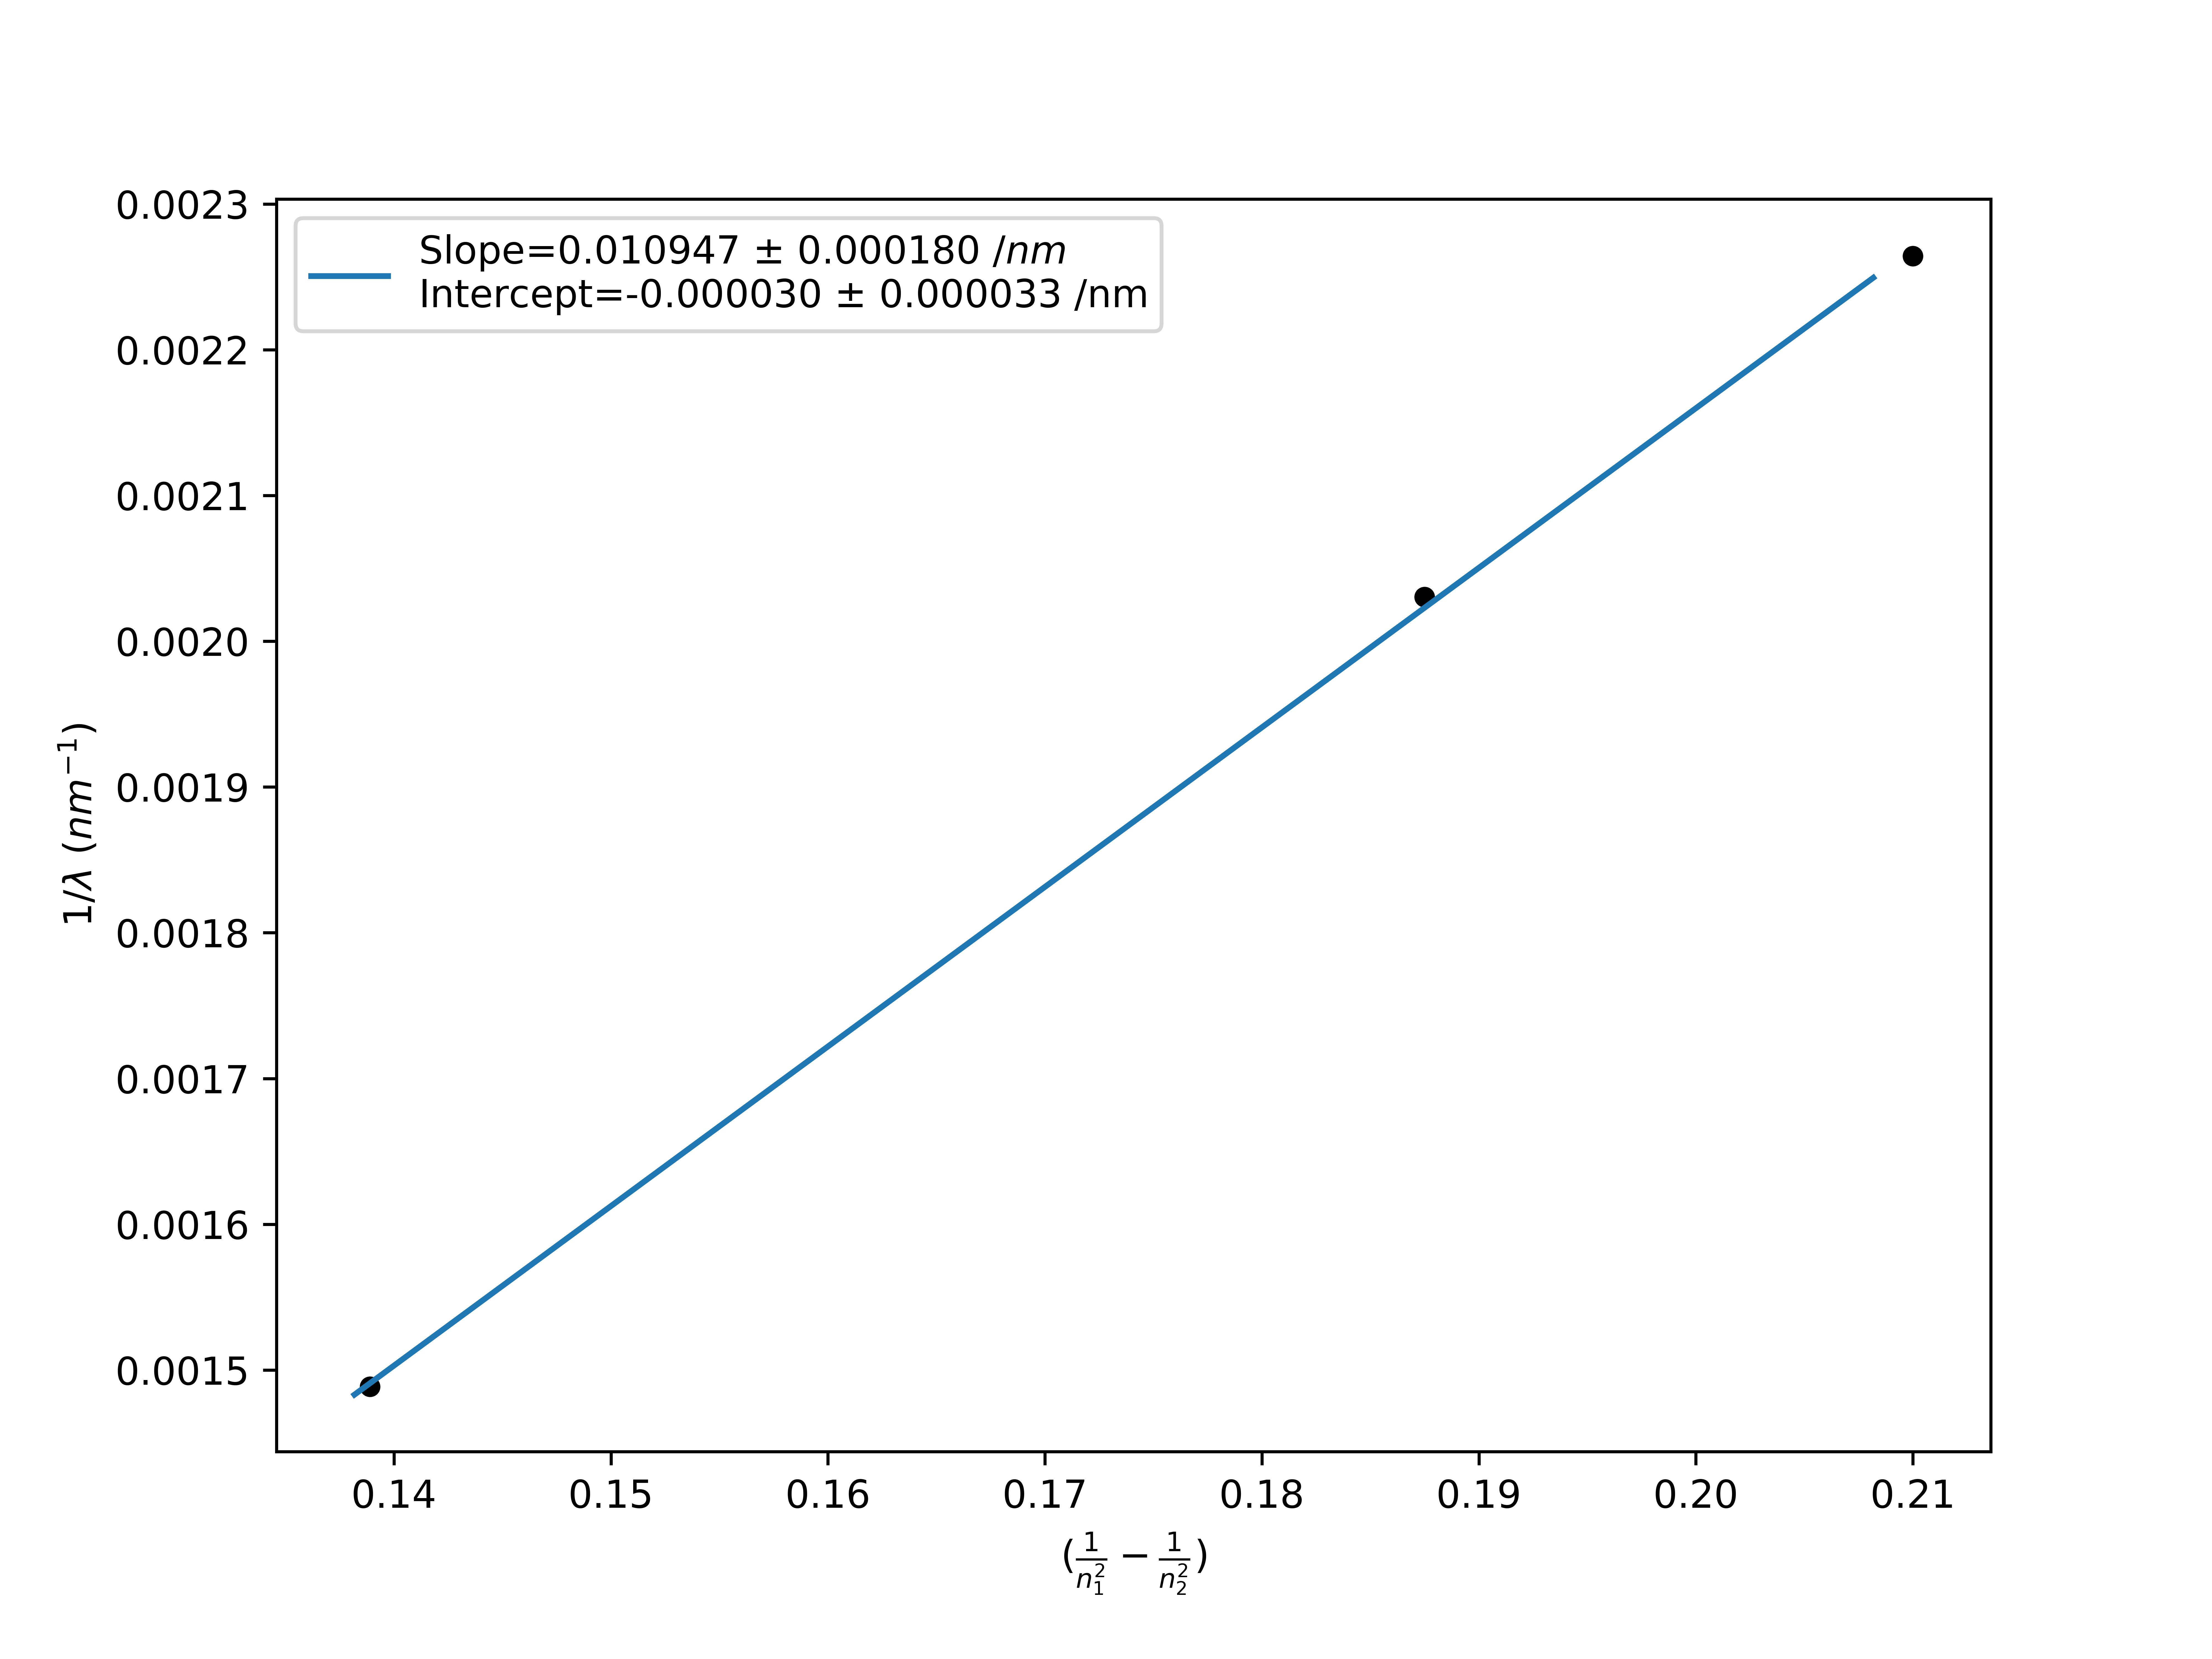
\includegraphics[width=8.5cm]{5} 
   \caption{Experimental setup in laboratory}
   \label{setup}
\end{figure}

\subsection{Precautions}
\begin{enumerate}
\item{Conduct the experiment in a quiet place devoid of electrical and mechanical disturbances. Even slightest disturbance could lead to misalignment of the data and readings.}
\item{Ensure that the current through Helmholtz coil is constant during observations.}
\item{Adjust the X and Y plate sensitivity of the oscilloscope to linear range.}
\item{Currents higher than 200 mA should not be allowed in Helmholtz coil as it would damage.}
\item{Ensure there is no overloading of the main line, as the peaks may not coincide since sinusoidal wave form of the mains may be distorted.}
\item{Use of AC stabiliser is discouraged as it may distort the sinusoidal wave form.}
\item{Use shielded cable to take the Y-output from the ESR spectrometer.}
\item{Ensure the cables are tightly connected to the channels.}
\end{enumerate}

\section{Analysis}

\begin{figure}[htbp] %  figure placement: here, top, bottom, or page
   \centering
   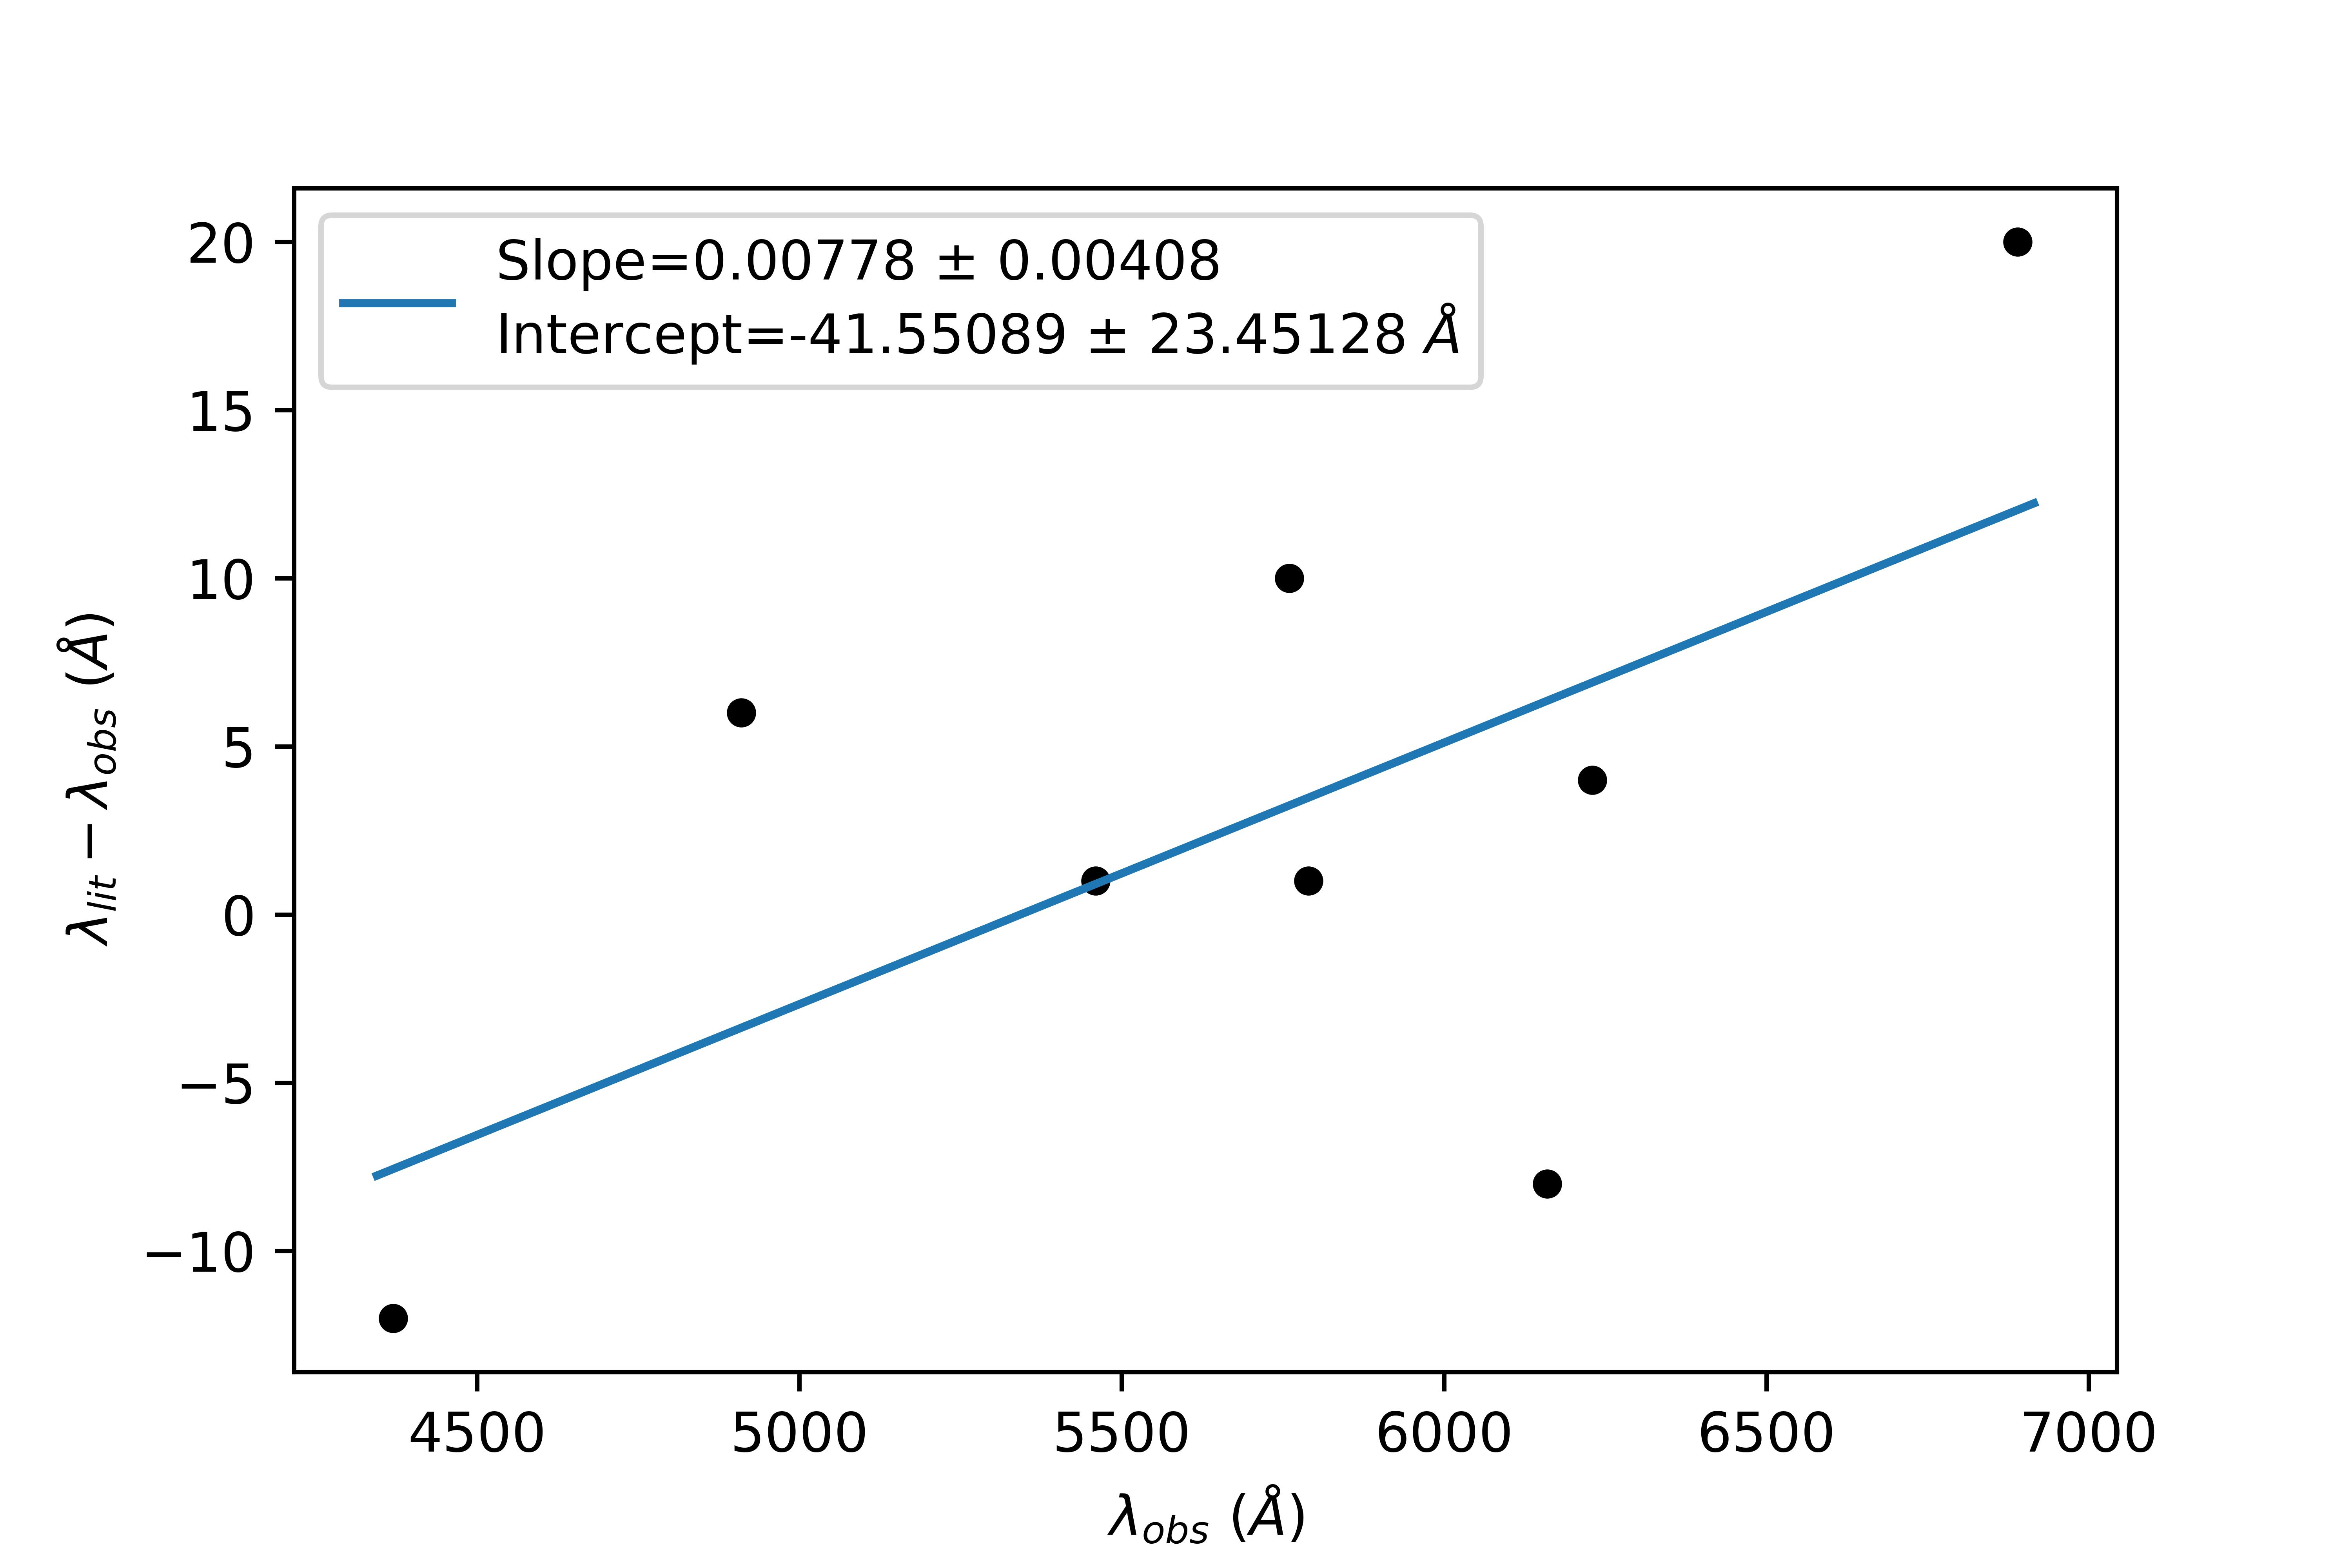
\includegraphics[width=8 cm, height=4 cm]{6} 
   \caption{Two peaks obtained after adjusting the phase}
   \label{lines}
\end{figure}

\begin{figure}[htbp] %  figure placement: here, top, bottom, or page
   \centering
   \includegraphics[scale=0.27]{9} 
   \caption{Plot of $Q$ versus 1/I for different frequencies}
   \label{g}
\end{figure}

The readings for current $I$ and $Q$ was taken for different frequencies and the graph was plot with $Q$ on the Y-scale and 1/$I$ on X-scale. For the frequency of 13.21 MHz, the slope QI is 2.884 ± 0.188 mm A, for frequency of 13.92 MHz, the QI is 3.382 ± 0.325 mm A, for frequency of 14.58 MHz, the QI is 3.500 ± 0.121 mm A,  for frequency of 15.16 MHz, the QI is 3.939 ± 0.206 mm A, for frequency of 15.85 MHz, the QI is 3.529 ± 0.113 mm A and for frequency of 16.14 MHz, the QI is m 3.771 ± 0.141 mm A. 
\newline

From equation (\ref{q1}) and (\ref{q2}), $H$ can be calculated from which $H_{pp}$ can be calculated to get $H_o$. Take the a=7.6 cm and n=500 for the Helmholtz coil used in laboratory. Therefore,  magnetic field at resonance frequency is 
\begin{equation}
H_o=H_{pp}.QI/P
\end{equation}
\newline
From equation (\ref{69}), we calculate the g factor as follows:
\begin{equation}
g=\frac{h\nu_o}{\mu_o.H_o}
\end{equation} 

where $h$ is Planck's constant, $\mu_{o}$ is Bohr's magneton, $\nu_o$ is resonance frequency. With the substitutions, we get $H_{pp}$=168 Gauss/A. $QI$ is obtained by the slope of the plot of $Q$ v/s $1/I$.
With the necessary substitutions for the constants and the frequency and slope we calculate g factor. The mean g factor obtained from all the frequencies is $1.300\pm0.068$. 

Comparing the experimental value of g with the standard value of g, 2.000. The experimental value of g deviates from the standard value because of instrumental errors, random errors. The experiment should be conducted in very quiet place which should be free from any fields interacting the apparatus. The instrumental errors contribute to the error, as it was experienced during the experiment. The mains should not be overloaded as the waveforms will be distorted, resulting in inaccurate value of Q. It should also be ensured that the current do not vary and remains constant during the experiment.

\section{Conclusion}
Electronic spin resonance was used to determine the Lande's factor, g for a free electron. We found g to b $1.300\pm0.068$ but the literature value is 2.0. We used 2,2 Diphenyl-1- picrylhydrazyl (DDPH) for the experiment since it is a free radical. The transitions could be induced between spin states by applying a magnetic field and then supply radio waves to it. We can see there is large error in the experimental values due to random errors.
Applications of electron magnetic spin resonance in solid state physics are of great importance. It is a very sensitive technique and has been applied in many fields such as paramagnetic ions in crystals, unpaired electron in semi-conductors and organic free radicals, colour centres, and radiation damage centres, ferro and anti-ferro magnetic materials. Pulsed ESR is used to control the state of electron spin qubits in materials such as diamond, silicon and Ga-As, in the field of quantum computing.

\section{References}
\begin{enumerate}
\item{\url{https://www.niser.ac.in/sps/sites/default/files/basic_page/ESR_manual.pdf}}
\item{\url{https://en.wikipedia.org/wiki/DPPH}}
\item{\url{http://www.nou.ac.in/econtent/Msc%20Chemistry%20Paper%20IX/MSc%20Chemistry%20Paper-IX%20Unit-6.pdf}}
\item{\url{https://en.wikipedia.org/wiki/Electron_paramagnetic_resonance}}
\item{\url{http://hyperphysics.phy-astr.gsu.edu/hbase/molecule/esr.html}}
\end{enumerate}

\end{document}